\begin{figure*}[t] 
	\begin{center} 
        \vspace{10pt}
		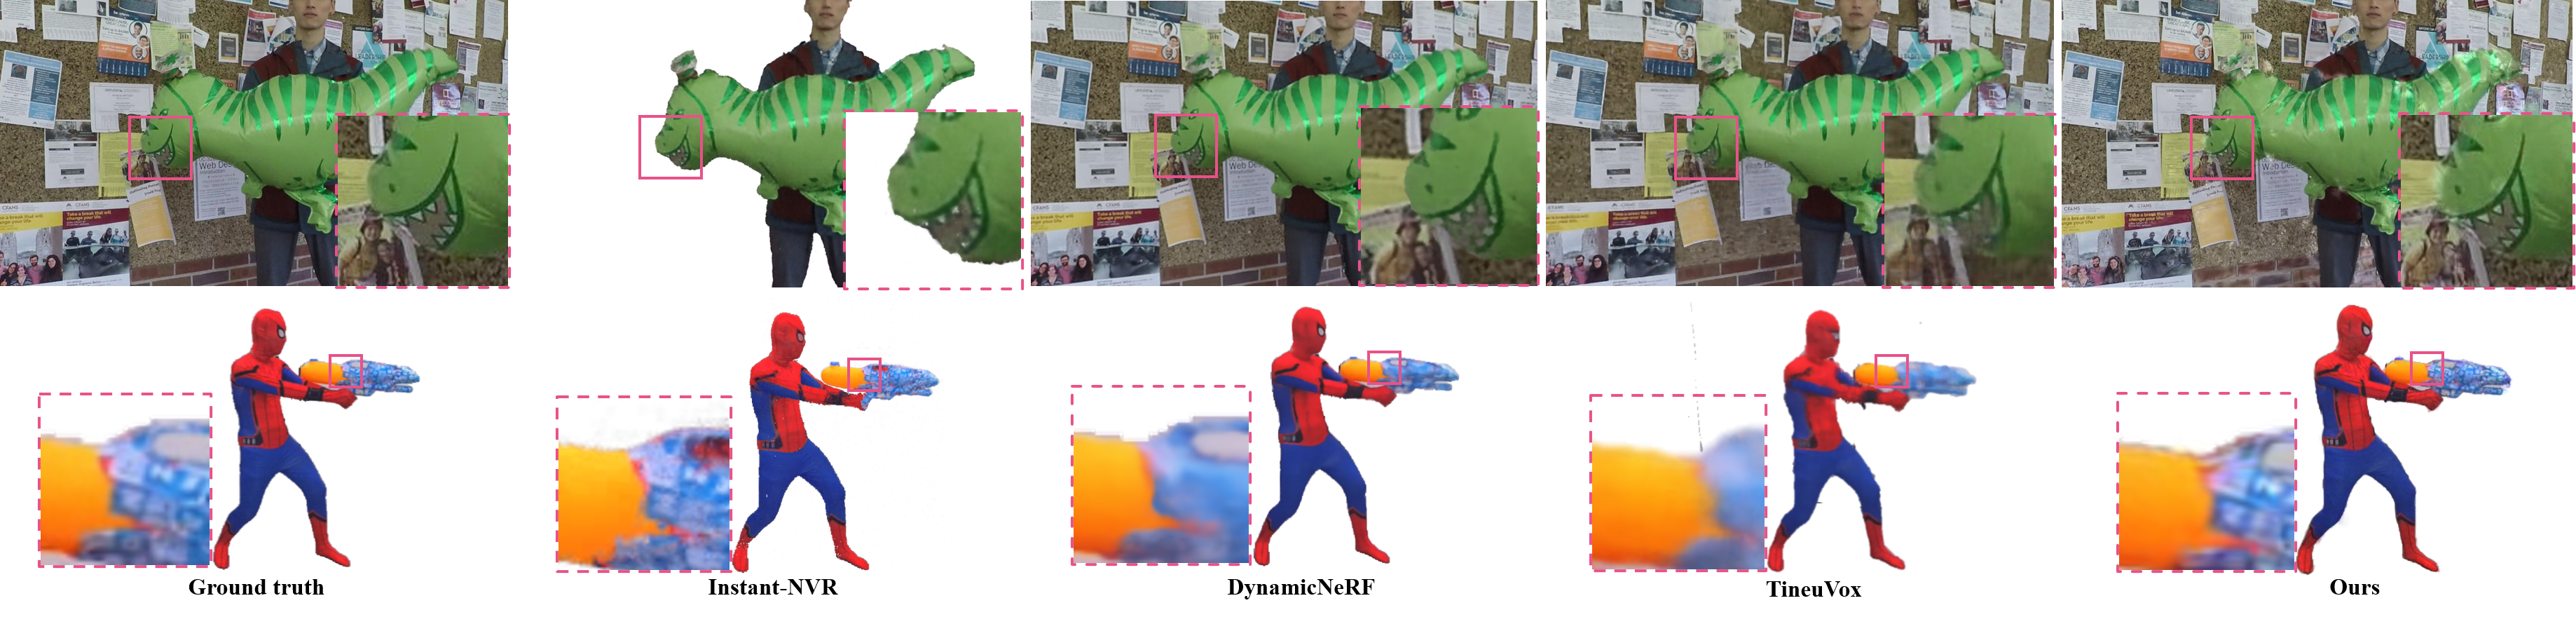
\includegraphics[width=\linewidth]{sec/fig/comparison.png} 
	\end{center} 
    \vspace{-15pt}
    \caption{Qualitative comparison against monocular dynamic scene reconstruction methods}
	\label{fig:comparison} 
\end{figure*} 

\section{Experiments}
\subsection{Ablation}
\noindent{\bf Flow Tracking Prior}
We conduct a qualitative ablation on the flow tracking prior to assess its impact on rendering results. As shown in Tab.~\ref{table:quantitative}, omitting the flow tracking prior and relying solely on the deform net tends to prolong the training time. In contrast, our full pipeline enhances the preprocessing of images to establish flow between frames. This approach integrates depth and optical flow, serving as an efficient initialization method for the deform net, aiming to expedite the optimization process.

% We conduct a qualitative ablation
% on the dual-graph and the regularization term to assess their
% impact on post-compression rendering results. As shown in
% Fig. 6, the removal of the coarse ED-graph prior typically
% causes severe artifacts. Excluding the Gaussian graph of-
% ten results in significant precision loss and unnatural render-
% ing. Regarding regularizers, the omission of Etemp usually
% triggers unrealistic artifacts post-compression. Meanwhile,
% the absence of Esmooth produces blurry results, with both
% leading to flickering in the video. Additionally, to evalu-
% ate the impact of the adaptive weight wi,t, we replace it
% with a fixed weight of 0.1. This adjustment generally leads
% to noticeable blurriness, especially in areas with significant
% movement. In contrast, our full pipeline generates spatially
% and temporally compact 4D Gaussians, maintaining high-
% fidelity rendering even after compression. The quantitative
% results are as demonstrated in Tab. 2, in which our full ap-
% proach achieves the highest accuracy.

% Without Flow Tracking: directly use deform net to construct 
% deformable gaussians
% • Ours-full: preprocess images to get flow between frames. 
% Utilizing depth and optical flow as an effective initialization 
% strategy for the deform net, aiming to expedite the 
% optimization process.
% • Experimental equipment: We completed the experiment 
% with 4 Nvidia 2080Ti graphics cards.

\begin{table}[t]
    \Huge
	\begin{center}
		\centering
		\caption{Quantitative evaluation of flow tracking prior.}
		\label{table:quantitative}
		\resizebox{0.45\textwidth}{!}{
			\begin{tabular}{l|c|c}
				\hline
				\hline
&Training (min) $\downarrow$ & PSNR(dB) $\uparrow$\\
\hline
Without Flow Tracking  &  93.23 & 31.65  \\
% \hline
Ours-full(before compression)     &  70.34 & 32.47  \\
% \hline
\hline
Ours-full(after compression)     &  70.64 & 32.30 \\
% \hline
\hline
\hline
			\end{tabular}
		}
		\vspace{-20pt}
	\end{center}
\end{table}


\begin{figure*}[t] 
    \centering 
    \includegraphics[width=\textwidth]{sec/fig/scale.png} 
    \vspace{-20pt}
    \caption{Comparison of residuals with and without the inclusion of scaling}
    \label{fig:scale_ablation}
\end{figure*}

\noindent{\bf Scaling}
In the Gaussian parameters (rotation, position, scaling) for shape and position, we found that optimizing the scaling parameter didn't notably improve rendering but increased training time. Consequently, in designing our deform-net, we omitted to optimize the Gaussian scaling. Results from training with and without scaling indicate a $9\%$ time difference (with scale: 102 min, without scale: 93 min).

Furthermore, the exclusion of the scaling parameter had a negligible impact on the rendering performance, with a marginal decrease in PSNR by just 0.05. Visual comparison in Figure~\ref{fig:scale_ablation} also confirms that the residual difference between the render result and ground truth is minimal, with or without the scaling parameter in the model.



% \begin{figure*}[t] 
% 	\begin{center} 
% 		\includegraphics[width=\linewidth]{sec/fig/pipeline.png} 
% 	\end{center} 
%     \vspace{-20pt}  
% % (a)我们的setting是RGBD monocular stream (b)对depth反投影产生初始点云初始化gaussians (c)利用flow between frames对gaussians进行warp,得到的warped gaussians作为先验进入deformable net(D-net)(d)D-net额外引入time作为输入估计当前的deltax,deltay,deltaz,deltar (e)对得到的gaussians利用RANS和quantization进行压缩
%     \caption{\noindent{\bf Overview of DynTCG.} (a) Our setting involves an RGBD monocular stream. (b) DynTCG performs back-projection on the depth to generate initial point clouds and initialize Gaussians. (c) Utilizing the flow between frames, we warp the Gaussians, and the resulting warped Gaussians are used as a prior input into the deformable network (D-net). (d) The D-net additionally introduces time as an input to estimate the current $\delta(x)$, $\delta(y)$, $\delta(z)$, and $\delta(r)$. (e) After training, the Gaussians are then compressed using RANSAC and quantization.}
% 	\label{fig:fig_2_overview} 
% 	\vspace{-8pt}
% \end{figure*} 


\noindent{\bf Residual Compensation}
As illustrated in Tab.~\ref{table:residual}, we allocate 46.23MB of storage for the 4D Gaussians of each frame before compression. Applying high-bit quantization (0-bit for motion and 9-bit for appearance) without residual compensation results in a storage requirement of 7.34MB. Using low-bit quantization (11-bit for motion and 7-bit for appearance), again without residual compensation, reduces storage to 3.23MB but compromises rendering quality. In contrast, applying the same low-bit quantization but with residual compensation significantly reduces storage needs to under 2MB per frame while maintaining the same level of rendering quality.
\begin{table}[b]
    \Huge
	\begin{center}
		\centering
		\caption{Quantitative evaluation of residual compression methods.}
		\label{table:residual}
		\resizebox{0.45\textwidth}{!}{
			\begin{tabular}{l|c|c}
				\hline
				\hline
& Per-frame Storage(MB) $\downarrow$ & PSNR(dB) $\uparrow$\\
\hline
Raw Point Cloud   &  46.23 & 32.47  \\
% \hline
High-bit Quantization    &  7.34 & 32.23  \\
% \hline
Low-bit Quantization    &  3.23 & 29.56  \\
% \hline
\hline
Ours Residual Encoding    &  1.35 & 32.30  \\
\hline
\hline
			\end{tabular}
		}
		\vspace{-20pt}
	\end{center}
\end{table}

% \begin{figure*}[t] 
% 	\begin{center} 
% 		\includegraphics[width=\linewidth]{sec/fig/encoding.png} 
% 	\end{center} 
%     \vspace{-20pt}
%     \caption{Illustration of residual encoding strategy for DynTCG.}
%     \label{fig:encoding}
% \end{figure*}
% \begin{figure}[t]
% 	\centering
% 	\includegraphics[width=\linewidth]{sec/fig/encoding.png}
% 	\vspace{-20pt}
% 	\caption{Illustration of residual encoding strategy for DynTCG.}
% 	\label{fig:encoding}
% \end{figure}
\subsection{Comparison}
We compare DynTCG with the methods including Instant-NVR\cite{jiang2023instantnvr}, DynamicNeRF\cite{gao2021dynamic}, and TineuVox\cite{Fang_2022} on Dynamic Scene Dataset and our captured data. As depicted in Fig~.\ref{fig:comparison}, we can observe that for areas with abundant texture and sharp edges, the reconstruction effect of Instant-NVR is mediocre, and its color prediction is also not very accurate. DynamicNeRF and Tinuvox show better overall object reconstruction, but their performance in texture detail is poor, resulting in significant blurring at the edges, to the extent that texture details become indiscernible. In contrast, our method DynTCG, based on Deformable 3D Gaussians, enhances its performance with depth map back-projection for point cloud re-projection constraints. Additionally, using Optical Flow Tracking as a prior provides a better initialization, leading to significantly improved results. Our method achieves better outcomes for complex textures, reconstructing them with greater clarity. Simultaneously, we also compare the average performance across different datasets in terms of PSNR, SSIM, and Per-frame Storage. It can be seen from the Tab.~\ref{table:Qualitativecomparison} that our metrics are superior to other algorithms in several aspects, further validating the robustness of our algorithm. The qualitative metrics prove that the rendered picture of our method surpasses other methods. What's more, the storage of our method can be reduced by about 90 percent compared with our methods, which ensures the easy preservation of each frame.
\begin{table}[t]
	\begin{center}
		\centering
		% \vspace{-25pt}
        \caption{
        Quantitative comparison of rendering results. Green and yellow cell colors indicate the best and the second-best results. %best and the second best results.
        }
		\resizebox{0.47\textwidth}{!}{
			\begin{tabular}{l|ccccc}
				\hline
				Method   &  PSNR $\uparrow$ & SSIM $\uparrow$ & Per-frame Storage(MB) $\downarrow$ \\
				\hline
                    Instant-NVR~\cite{jiang2023instantnvr} & 28.82 & 0.976 & 24.16 \\
				DynamicNeRF~\cite{gao2021dynamic}\qquad\qquad & 26.65 & 0.8452 & 21.5 \\
			    TineuVox~\cite{Fang_2022}     & 24.71 & 0.813 &  \secondBestCellColor{11.38} \\
    		\hline

                Ours(Before Compression)  & \bestCellColor{\textbf{32.47}} & \bestCellColor{\textbf{0.989}} & \textbf{43.42}\\
                Ours(After Compression) & \secondBestCellColor{\textbf{32.30}} & \secondBestCellColor{\textbf{0.983}} & \bestCellColor{\textbf{1.648}}\\
				\hline
			\end{tabular}
            }
		\label{table:Qualitativecomparison}
    
    		\vspace{-25pt}
	\end{center}
\end{table}
